\documentclass{llncs}
\usepackage[colorlinks,allcolors=blue]{hyperref}
\usepackage[T1]{fontenc}
\usepackage{listings}
\usepackage{graphicx}
\usepackage{amsfonts}
\usepackage{verbatim}
\usepackage{cite}

\graphicspath{{./images/}}

\begin{document}

    \title{Quality assurance of digital twins -- An experience report in the automotive industry}

    \author{Georg Hackenberg\inst{1}
    \and
    Alican Tüzün\inst{1}
    }
    \institute{School of Engineering\\
    University of Applied Sciences Upper Austria\\
    4600 Wels, Upper Austria, Austria\\
    \email{lncs@springer.com}}
    
    \maketitle

    \begin{abstract}
        Digital twins are becoming more and more important for the efficient and effective development and operation of cyber-physical systems.
        However, digital twins are only useful if they reflect the real-world system accurately enough, i.e.\ their quality is high enough.
        This claim entails the question, of what the term quality in the context of digital twins means and how it can be measured.
        In this article, we present our experience with the quality assurance of a digital twin for an assembly line in the automotive industry.
        We explain our preliminary definition of digital twin quality, which we derive from classical quality models for general software systems.
        Furthermore, we describe quality issues, which we were able to detect in a digital twin of an assembly line in the automotive industry.
        Finally, we conclude how to leverage our experience in different contexts and how to generalize the underlying approaches.
    \end{abstract}

    \section{Introduction}\label{section:introduction}
    
    The notion of the digital twin, which has gained popularity in 
    recent years, is often subject to vague and ambiguous envisions\cite{Review1}.
    The mispresenting this notion began with the physical twin of the Apollo 13 spacecraft. 
    The twin of Apollo 13 was merely a tangible replication of the spacecraft that has been utilised in the physical simulations. 
    Even though the digital aspect was expected to be present, there wasn't\cite{GrievesApollo13}.
    Another physical twin is the historic D-day map (also known as the Big Board) in Southwick House England, 
    which was used simultaneously before and during operation, can be argued to be similar. 
    The board was a twin of the operation, and it included model of battalions and ships that reflected the actual 
    locations of the corresponding formations. Furthermore, synchronisation was 
    implemented to give directives from the real system to control the operation 
    flow and to update the physical twin state\cite{AMRC}.
    In contrast, a digital twin is a virtual counterpart of a real system, which should 
    be synchronized with a selected frequency and fidelity\cite{Review1,Review2,digitaltwinconsortium2022}.
    
    The envision of digital twin emerged from Grieves'es conceptual model, which was called mirrored spaces model in 2002~\cite{Originsofdigitaltwinconcept},
    and later referenced in 2005 journal article~\cite{2005JournayArticle}. 
    Furthermore, he introduced the information mirroring model, which was his ideal product lifecycle management tool with only one goal. 
    The goal was to gather as much as  information about the real system to minimize the waste of system's sources such as energy, 
    time and material. Initially this model had four main parts with real system, 
    virtual system, connection between the real and virtual system and virtual simulations\cite{GrievesPLMBook}. 
    Later, Grieves removed the latter, in order to simplify the model\cite{Originsofdigitaltwinconcept}.Furthermore, after co-authoring with the Vicker's in 2010, 
    Grieves decided to use the NASA invented Digital Twin word, instead of information mirroring model\cite{Originsofdigitaltwinconcept}.
        
    Digital twins are highly intricate and adaptable systems that possess the capability to not only respond to environmental 
    changes but also modify their internal structure \cite{ZHANGUPDATEMETHOD,MobusSystemTheory}. Therefore, ascertaining a 
    requisite level of quality for the construction of a digital twin is an arduous undertaking.

    FELICE is a complex system which  addresses a critical problem in robotics which is the effective integration of human and robot abilities in a collaborative setting. 
    This challenge requires the development of sophisticated algorithms and techniques that facilitate seamless communication, cooperation, and coordination between humans and robotic agents. 
    By addressing this issue, FELICE tries to represent a significant advancement in the field of robotics and has the potential to enhance the effectiveness and efficiency of a wide range of 
    human-robot collaborative tasks with the consideration of safety~\cite{FELICE}.

    Main purpose of this study is to identify the quality attributes and inspect several artifacts 
    with these to evaluate the quality of the digital twin for the FELICE project, 
    which is currently in the design phase~\cite{FELICE}. These artifacts included process videos showing the current 
    assembly procedure, a scope definition, a requirements specification, a general and operational conceptual model, 
    and a discrete event simulation module. We assessed the quality of these artifacts based on five crucial quality attributes: correctness, completeness, fidelity, efficiency, and evolvability.

    %%
    %%\subsection{Research objective}
    %%Find an approach to assess the quality of Digital twins~\cite{Jones2020}

    %%\subsection{Research question}\label{section: Research Questions}
    %%What is the quality of digital twins?
    %%What is the state art of digital twin quality?

    %%\subsection{Research methodology}
    %%TODO

    \section{State of the art on quality}
    Oxford English Dictionary describes the word quality  either as a noun or as an adjective. 
    The adjective form indicates, a high standard or excellence. For example, the phrase quality products implies 
    that quality adds a high standard state to the product. There are several definitions which describes a quality 
    as a noun,however the impactful definition is the quality as a standard of an entity which is measured against the 
    different or the similar entities\cite{OxfordDictionary}.This definition clearly shows the relativity of quality.In addition, quality be defined 
    as the degree to which a set of inherent properties of an entity fulfills the given requirements~\cite{ISO9000}.    

    \subsection{Product quality and Management}
    A product is a tangible or intangible system that satisfies the needs or wants of a customer. It could be a physical system like a car, or an abstract system, like a digital twin. 
    Regarding product quality, there are two different aspects~\cite{GrievesPLMBook}.
    First, quality is an attribute of a product, which meets product specifications. Specifications are mostly defined by the supra-systems subsystems, such as by the stakeholders within the supra-system,  If the stakeholders' expectations, or needs, are met, we can consider high quality.
    The ability to execute to a specific usage standard is the second facet of product quality. Since this standardization is usually not controllable, unlike the first, the system's quality will be determined by how the implied or obligatory standards are fulfilled.

    Quality management is a management type, which has an interest in Quality, and quality assurance is one of the parts of quality management, 
    which focuses on providing fidelity that quality requirements will be fulfilled. This means that quality assurance is a subsystem of quality management.

    Quality management systems(QMS) are functioning to plan and execute the organizations quality policies and goals. 
    Examples of such systems can be a standard like ISO 9001 which can provide a framework for an organization, or a data-driven methodology such  as Six-Sigma to reduce defects and improve efficiency. 
    This concepts  are not new, for example ISO 9001 standard has been established in 1987, and still being regularly updated ~\cite{ISO9001DebunkingtheMyth}. 

    \subsection{Software quality}
    Software is a combination of programs and data which can be used by the virtual 
    systems as well as  a physical system like a computer system. In contrast a hardware 
    is a physical subsystem of a computer system\cite{OxfordDictionary}. 

    Software Quality is determined by how well software fulfill the requirements that were set. However, those requirements  
    not always reflect what the stakeholders actually need, hence the quality depends how accurately this requirements were set \cite{IEE730-2014}. 
    As a result, functional suitability, performance efficiency, compatibility, usability, reliability, security, maintainability 
    and portability are the standartized  eight attributes that measure software quality \cite{ISO/IEC:25010}.
    
    Software quality management techniques comes from already used manufacturing techniques in the  industries. For example the  product quality assurance has been used as a software quality management activity with some modifications. For example, in the manufacturing, products will never exactly meet a specification, due to errors in the machining which results in some tolerance area. But in the software systems, or more precise in the virtual systems, it's most of the time not the case. Also its nearly imposible to conclude that, 
    the software product is fully meet its speficiations. 
    Hence, most of the quality assesments are subjective process and as a result, the quality attributes should be inspected subjectively \cite{SoftwareEngineering}.  

    \subsection{Simulation Quality}
    Simulation models are not merely virtual systems; they are also abstracted systems, 
    which are nothing more than imitations or, to be more precise, abstractions of the real systems. 
    In fact, everyday, simulation of the real systems occurs in the human brain when prediction of the future outcome or  about the 
    past state of some occured event required\cite{MobusSystemTheory}. However, most of the simulation processeses are computer 
    based with software programs. Consequently, the idea of simulation software programs emerges. 
    For example, ANSYS\cite{Ansys}, ABAQUS\cite{Abaqus}, and AnyLogic\cite{AnyLogic} are examples of these simulation software programs. 

    Validation and verification is used to evaluate the quality characteristics of the simulation 
    model \cite{StewartSimulation,VerificationValidationSergent,OsmanBalci}. 
    Validation is the process of evaluating the simulation quality of the model in comparison to 
    the real system from the perspective of the model's intended applications.
    On the other hand, verification is a procedure to 
    evaluate a simulation model's implementation and its associated 
    data concerning the conceptual description and specifications of the 
    model developer\cite{StewartSimulation,VerificationValidationSergent}.

    \subsection{Digital twin quality}
    To analyze the state of the digital twin quality, a literature analysis was executed. 
    The analysis especially focused on how the digital twin quality is mentioned and assessed within the academic dissertations.

    \subsubsection*{Literature Search Methodology}
    To conduct a thorough literature review on digital twin publications, tools such as Google Scholar and Scopus are utilized. Due to the vast amount of available literature, it is necessary to narrow down the scope of the research. 
    Therefore, a multi-level filtering algorithm is employed to refine the search results.

    The first level of filtering for the literature review on digital twin publications involves specific criteria. These include that dissertations must be written in English and 
    published in a journal or conference, and that the search term must be an exact match. To execute this initial filtration, 
    the following queries are used for Google Scholar and Scopus respectively: "search term" and ALL ("digital twin quality") AND (LIMIT-TO (LANGUAGE, "English")).

    After the initial filtering, a second level of manual investigation is necessary. The following criteria are used for this level of filtering:    
    \begin{itemize}
        \item  Eliminating duplicates
        \item  Removing dissertations that are not in English
        \item  Ensuring that selected dissertations have a proper literature review
        \item  Ensuring that abstract and conclusion are relevant to the search term
    \end{itemize}

    If an interesting dissertation(s) would be found during the reading, it will be checked again with the initial filter.

    \subsubsection*{Literature Search Result}
    The search for "digital twin quality" initially resulted in 41 hits on Google Scholar and 3 on Scopus. 
    After the second level of filtering, 6 duplicate dissertations were removed and 10 dissertations that were not in English were also eliminated. 
    This left only 9 dissertations that met all the criteria and were reviewed.

    The search for "digital twin verification" initially resulted in 19 hits on Google Scholar and none on Scopus. 
    After the second level of filtering, one duplicate dissertation was removed and two dissertations that were not in 
    English were also eliminated. As a result, all dissertations were rejected.

    The search for "digital twin validation" initially resulted in 59 hits on Google Scholar and none on Scopus. 
    After the second level of filtering, 4 duplicate dissertations were removed and 4 
    dissertations that were not in English were also eliminated. This left only 8 dissertations that met all the criteria and were reviewed.
    
    After a thorough review of 17 research papers, a number of significant findings were revealed.
    
    First, it was noted that Shcherba et al.  focus on the importance of model quality as an observation for a digital twin subsystem. 
    However, they acknowledged that the quality assessment of the digital twin cannot solely rely on models~\cite{Shcherba}. 

    He Zhang et al.  developed a consistency evaluation approach for digital twin models, which can be used to assess their quality. 
    The authors also discuss essential concepts, such as consistency between real and virtual systems and ultra-fidelity models. 
    This article emphasizes the improvement of the service component of the digital twin~\cite{ZHANGEVALUATIONMETHOD}.

    He Zhang et al. introduced the updating method for digital twin models in yet another insightful article.
    Once more, the accuracy and coherence of the model concepts were addressed~\cite{ZHANGUPDATEMETHOD}.

    Selch et al.  present a machine-learning approach based on Bayesian networks to track the quality of the digital twin. 
    The unique aspect of this study is that the authors determine the contributions of subsystems to forecast the overall quality of the digital twin, 
    rather than just analyzing it as a single system. The digital couplings, which are linkages between the subsystems, are also identified as a source of extra uncertainty. 
    However, since only one digital twin has been used in practice, multiple subsystem digital twins have not been validated~\cite{QualityMonitoringofCoupledDigitalTwins}.

    Additionally, the stability of digital twin models was assessed by another study using the Kolmogorov-Smirnov statistical test, 
    which measures the degree of similarity between the probability distribution of the model's predictions and the distribution of the actual data~\cite{RadarDigitalTwin}.

    Edward Y. Hua et al. identify five open problems with digital twin model validation, including modeling realism, data uncertainty, system dynamics, use-case alignment, and reporting invalid modes. To address these challenges, the authors propose a digital-twin model validation framework. The paper also highlights three areas for future research, 
    including uncertainty and sensitivity analysis, model validation of system-of-systems, and combining expert knowledge and collected data ~\cite{ValidationofDigitalTwins}. 

    Finally, Shotaro Hamato et al.  demonstrated successful real-time anomaly detection using the Unscented Kalman Filter with the digital twin model. 
    However, determining the appropriate threshold for anomaly detection remains an issue~\cite{JapeneseKalmanFilterCorrectness}.

    Overall, these studies provide valuable insights into various aspects of digital twin quality assessment, 
    including model consistency, stability, and validation, as well as machine learning-based approaches and real-time anomaly detection. 
    However, the identified open problems, including modeling realism, data uncertainty, system dynamics, use-case alignment, and reporting invalid modes, 
    call for further research in the field to improve the quality and reliability of digital twins. Moreover, 
    the lack of well-defined quality parameters for digital twins poses a significant challenge in ensuring their quality,
    which necessitates the development of appropriate quality metrics and standards for digital twins.

    \section{Methods}
    Based on the theoretical background, we have opted for a methodology that comprises two components: 
    \begin{itemize}
        \item Manual Reviews
        \item Utilization of quality standards in conjunction with dictionary definitions of the quality attributes that will be employed
    \end{itemize}

    \subsection{Manual Reviews}
    We presented the results of the comprehensive manual reviews 
    conducted to evaluate the quality of digital twin artifacts during 
    the initial stages of the FELICE project. The current stage of review 
    encompasses five key artifacts, including process videos displaying the 
    current assembly procedure without an adaptive workstation and cobot, 
    a scope definition outlining the objects on the shop floor requiring tracking or twinning, 
    a requirements specification summarizing functional and non-functional requirements for the digital twin, 
    a general and an operational conceptual model elucidating the high-level structure of the assembly procedure, 
    and a discrete event simulation module that implements the structures prescribed by the conceptual models.

    \subsection{Quality Standards and Dictionary}
    We consolidated our findings from various standards, including ISO/IEC:25010, 
    IEE730-2014, ISO9000, ISO9001, and the Oxford dictionary, in order to establish clear 
    and precise definitions for the attributes used in assessing digital twin quality.\cite{ISO9000,ISO90012015,ISO/IEC:25010,IEE730-2014,OxfordDictionary}.
    
    \section{Digital Twin Quality Attributes and Results}
    
    \subsection*{First criterion: Correctness}
    Correctness is a  derived word from the adjective correct, which means that something is error-free regarding a fact or truth~\cite{OxfordDictionary}. 
    In the context of the digital twins, our fact or truth is a real system hence, correctness is a grade of quality, that indicates an error between the real system and a digital twin system.
    Meanwhile, the quality of being correct is described by the term accuracy. Another important word is precision, 
    which refers to the ability to be precise and accurate\cite{OxfordDictionary}. 
    From a technical standpoint, we use precision in mathematics by the number of provided digits. 
    For instance, binary64 has 53 significant digits while binary32 has 24, displaying the precision of the structure~\cite{IEE754}.  
    
    \subsection*{Second criterion: Completeness}
    According to the Oxford Dictionary, complete can be an adjective, an attribute, or  a verb with an object\cite{OxfordDictionary}. 
    When used as an adjective, it describes something 
    as having all the necessary or appropriate parts. To evaluate the completeness of a digital twin, 
    one must first analyze and synthesize the real system to identify subsystems and their relations with related systems in the supra-system. 
    After this initial analysis, completeness can be assessed by comparing the subsystems and relations of the real world with those of the digital twin.


    \subsection*{Third criterion: Fidelity}
    The concept of fidelity has garnered significant attention in recent years and continues to be an important area of research in digital twins.
    In the context of digital twins, Fidelity refers to the degree of exactness with which the real system is copied and represented.
    Low-fidelity indicates a simplified representation, while high-fidelity refers to an accurate and detailed representation of the real system.
    This quality attribute plays a crucial role in evaluating the effectiveness of digital twins in accurately capturing the behavior and properties 
    of real-world systems. 

    \subsubsection*{Fidelity vs Correctness}
    Correctness is a functional quality attribute, which assesses the behavior of the digital twin systems, 
    by how accurately the results with the given precision match the behavior of the real system or more
    specifically outputs with the same given inputs. 
    This quality attribute focuses on the behavior of the system.
    On the other hand, fidelity is another quality attribute to consider. 
    It deals with the level of exactness and detail in the digital twin system's representation. 
    Fidelity concerns itself, with how the digital-twin system is exactly relative to the real system with a certain level of detail, which is more to do with the depiction or representation of the digital twin systems, rather than their behavior of them.

    \subsection*{Fourth criterion: Efficiency}
    Efficiency refers to the quality of being efficient, and efficiency can be explained as achieving maximum productivity with minimum wasted effort or expense. 
    The concept of efficiency is tightly coupled with productivity, which refers to the quality of being productive. The word productive can be explained as producing or being able to produce large amounts of goods~\cite{OxfordDictionary}.
    For example, time efficiency indicates that,  with less amount of time as an input, more output with the minimum waste during the process is desired. Goods of the digital twin are nothing but information, 
    which Grieves first indicated with his Information Mirror Model~\cite{GrievesPLMBook}. So to assess the efficiency, one should inspect the sinks and sources of the digital twin system, to identify the waste, expense and productivity. 

    \subsection*{Fifth criterion: Evolvability}
    A system's capability to enhance its suitability to its environment through alterations to both its internal and functional structure is referred to as evolvability. Another term used to describe the response to changes in the environment is adaptability. 
    However, this concept differs from evolvability in that it only affects a system's internal or functional structure temporarily. In contrast, evolvable systems undergo definite changes in their structures.  
    For instance, a digital twin, which is a virtual system, can be designed to be more flexible and scalable, allowing for easy updates and the addition of new features. 
    These updates and new features will result in definite changes to the structure of the system. On the other hand, a responsive web design is an adaptable system, capable of adjusting its size and layout depending on the user's hardware. 
    As we have seen in~\cite{ZHANGUPDATEMETHOD}, the update method shows that digital twins are evolvable systems,
    hence this attribute should be considered when the digital twin's quality is inspected. To assess the evolvability attribute, scalability analysis, reusability analysis, modifiability analysis, testability analysis, and maintainability analysis can be performed. 


    \begin{figure}[htbp]
        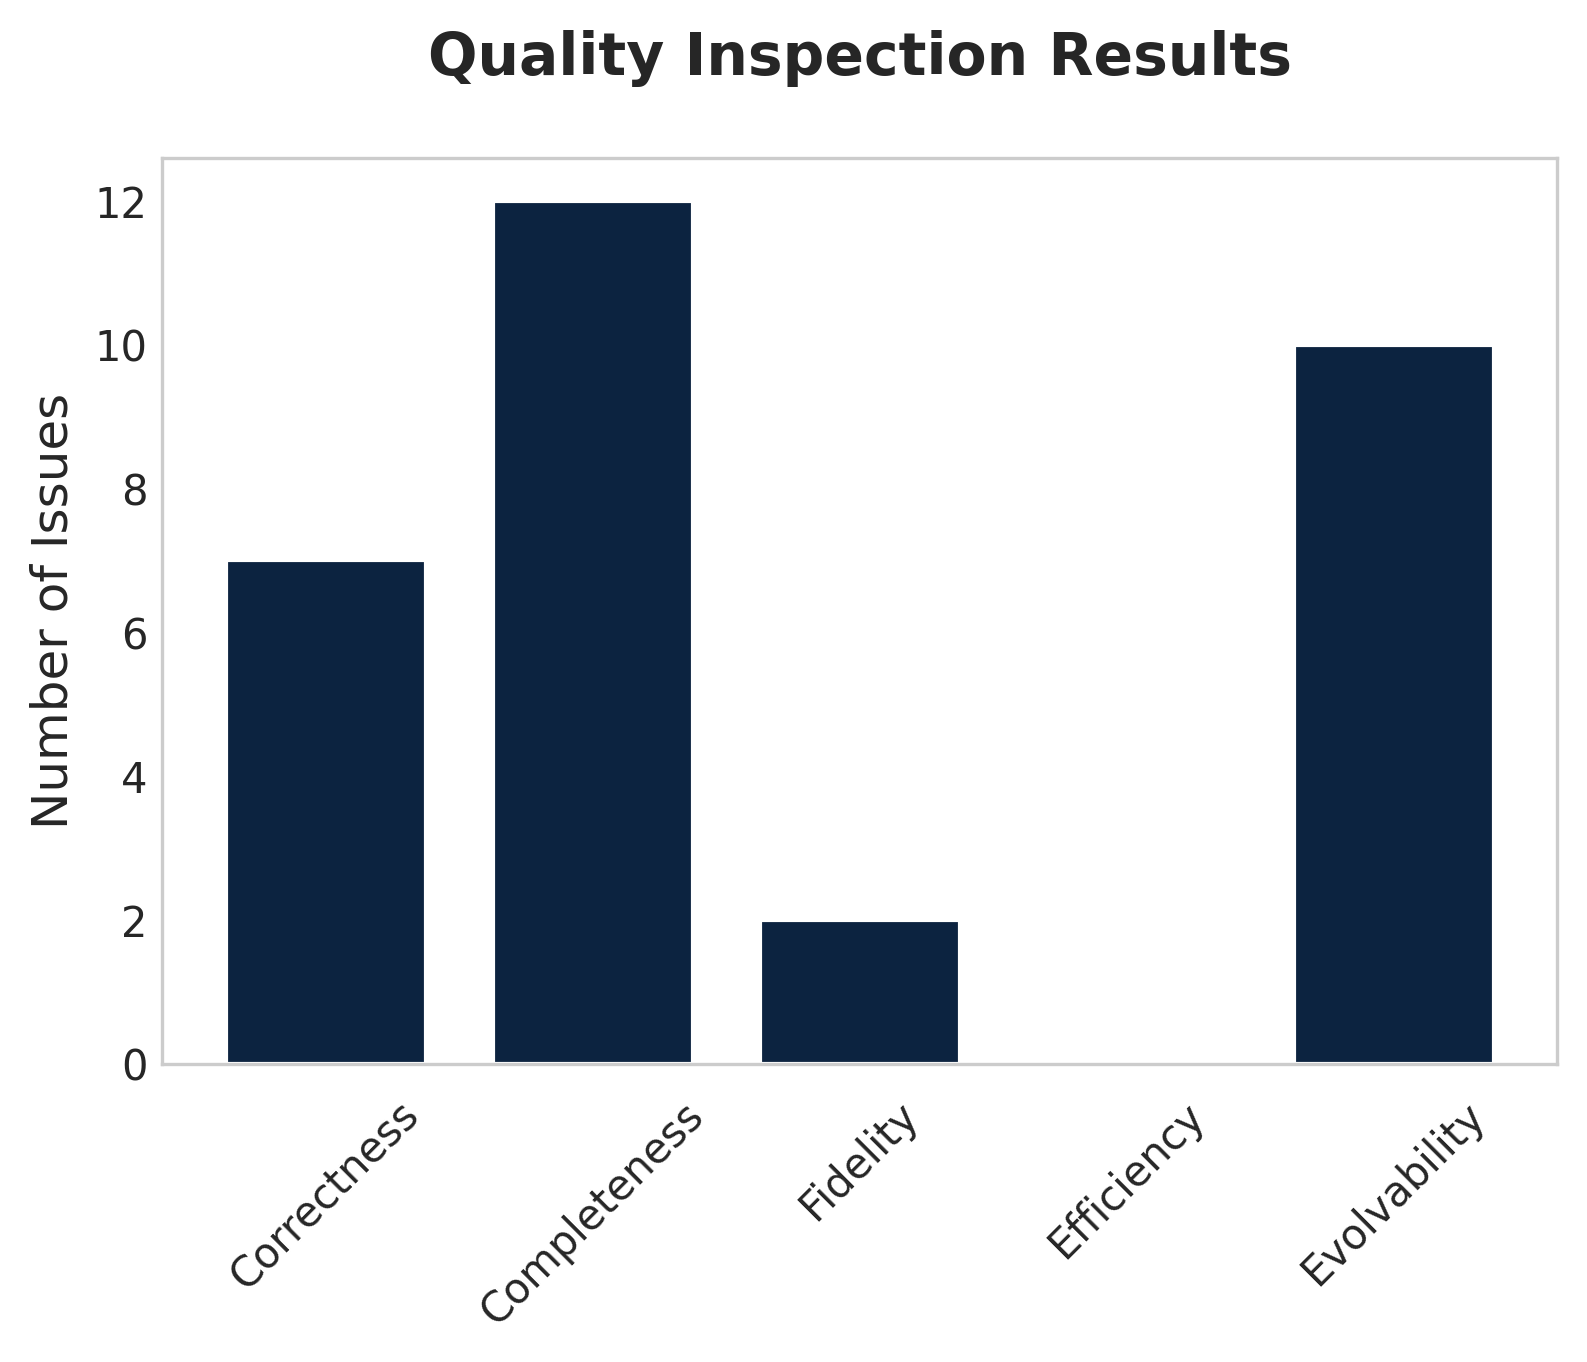
\includegraphics[scale=0.75]{quality_inspection_results.png}
        \caption{Overall Quality Inspection Results}
        \label{fig:QualityInspectonResults}

    \end{figure}\begin{figure}[htbp]
        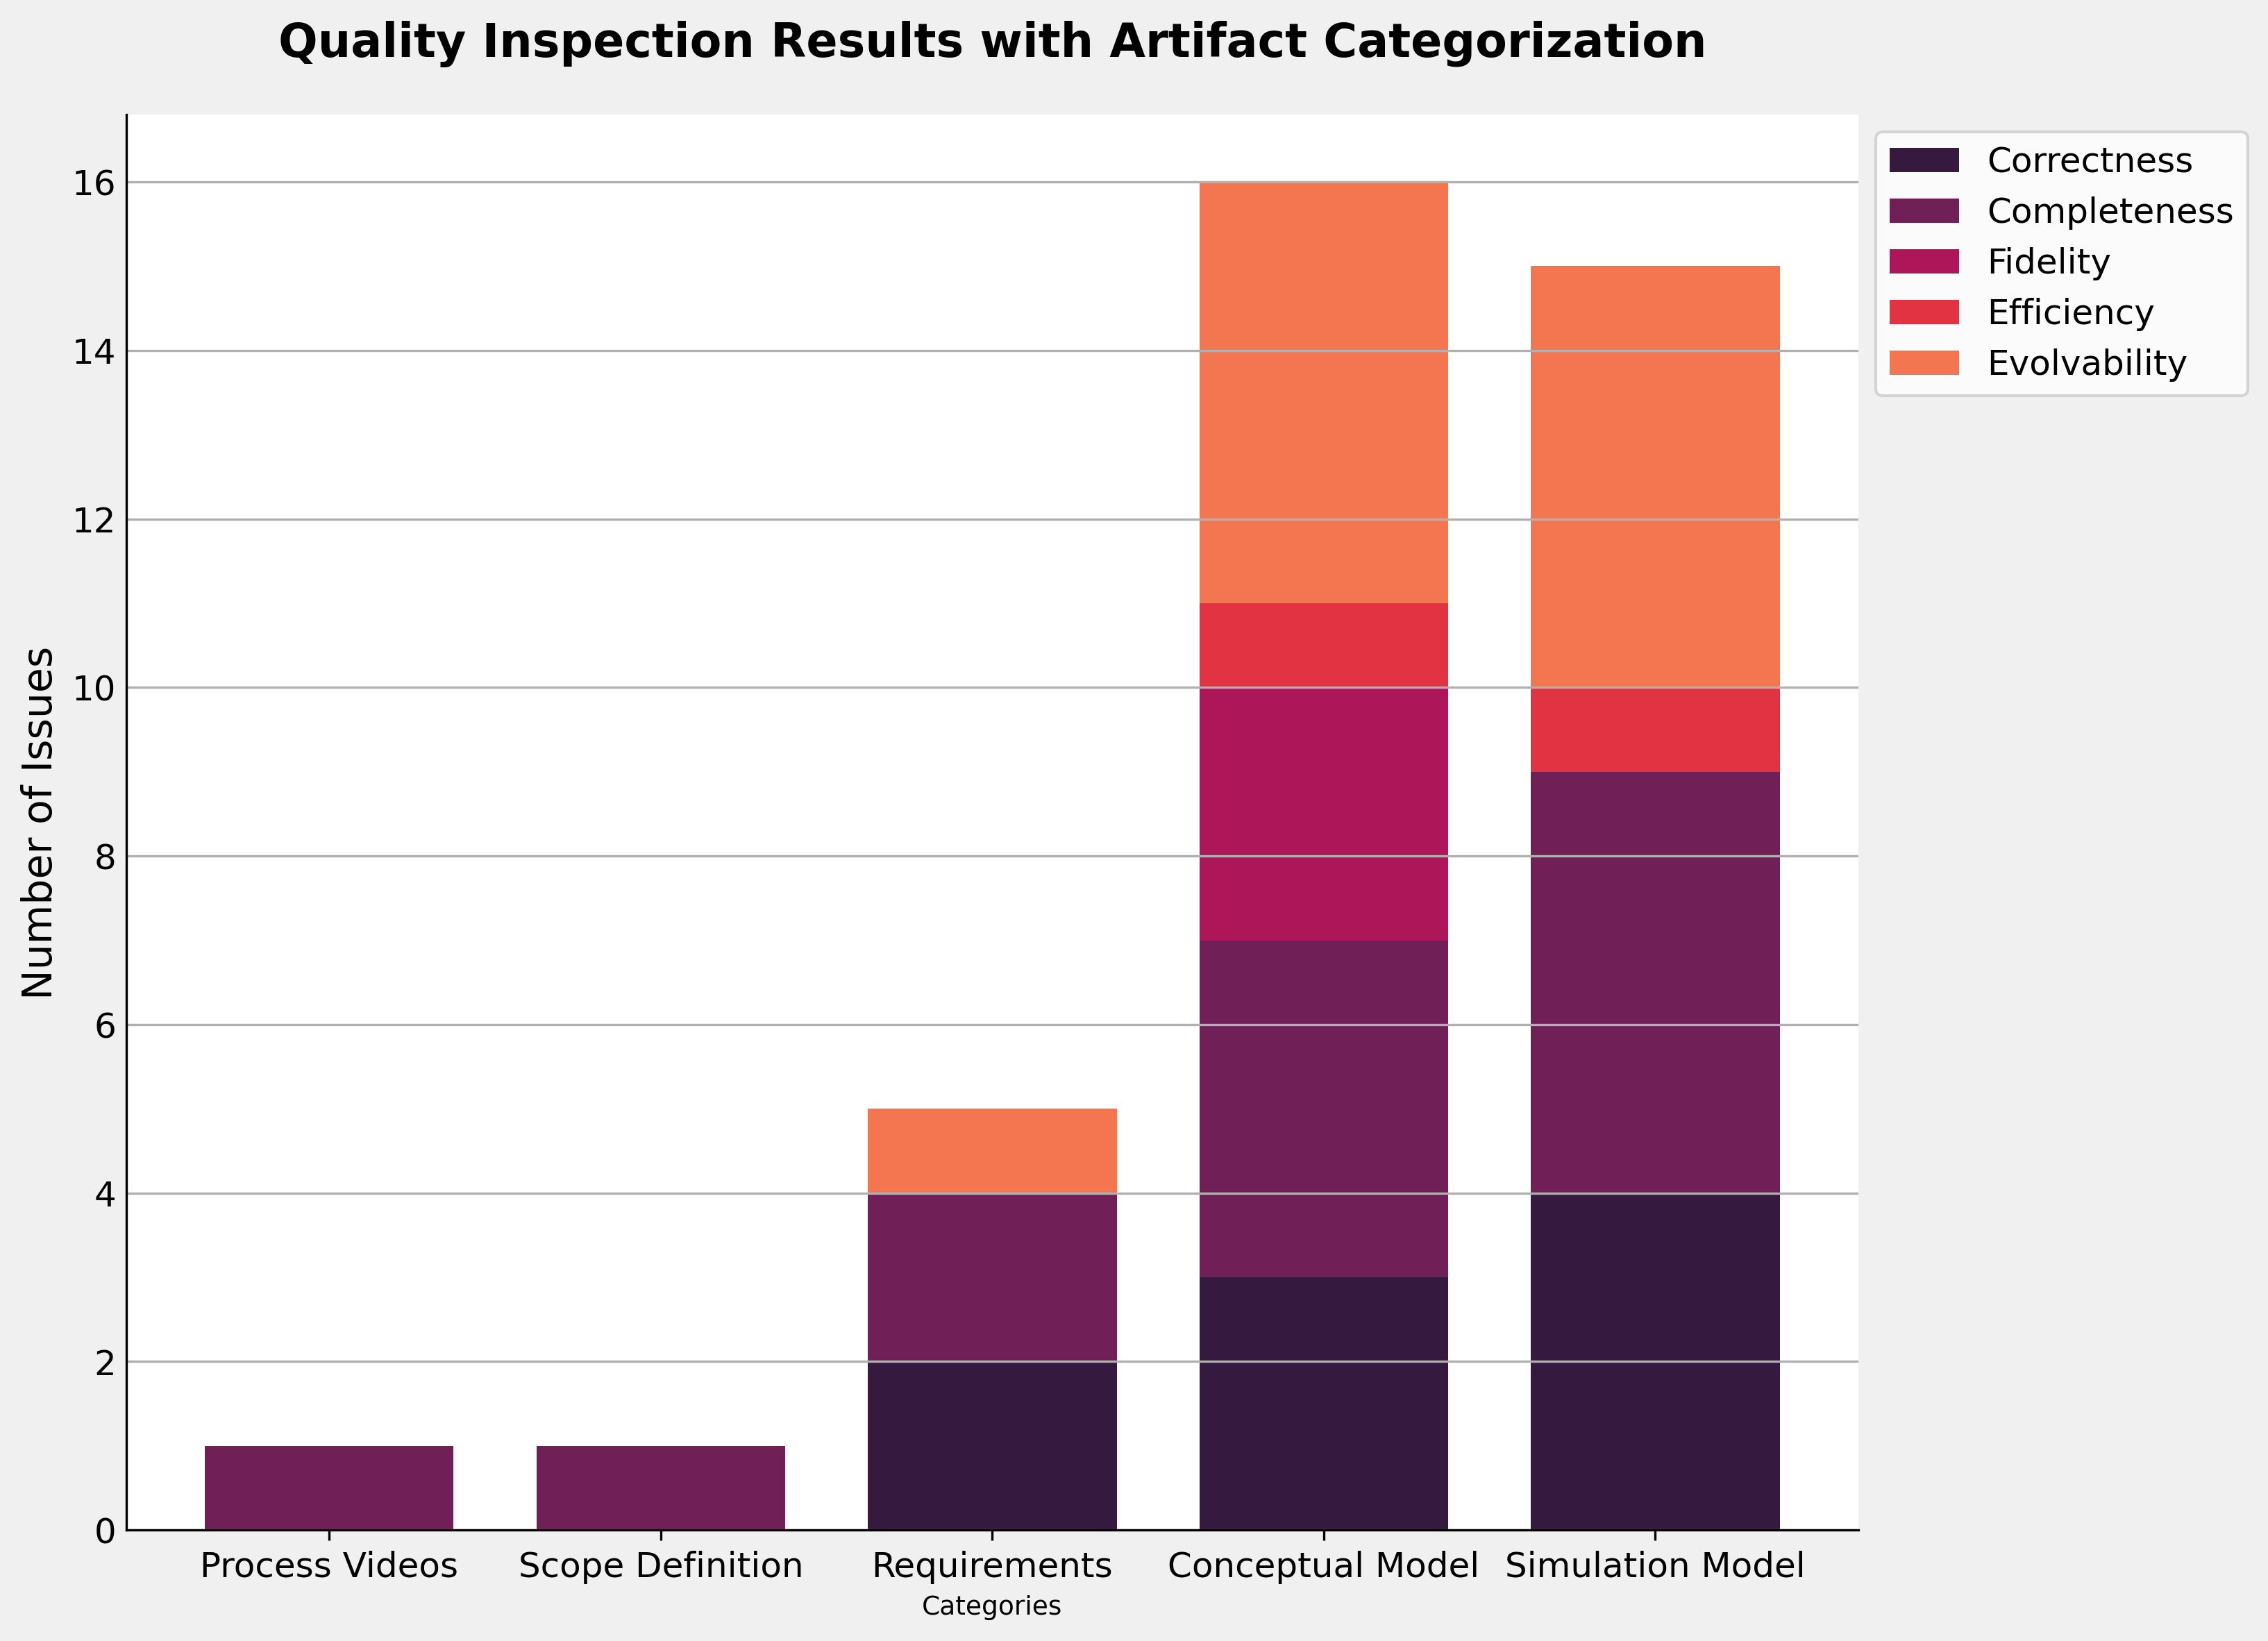
\includegraphics[scale = 0.45]{quality_inspection_results_with_artifacts.png}
        \caption{ Quality Inspection Results Categorized with Artifacts}
        \label{fig:QualityInspectonResultsWithArtifacts}
    \end{figure}

    As can be seen in Figures ~\ref{fig:QualityInspectonResults} and ~\ref{fig:QualityInspectonResultsWithArtifacts}, based on our inspection of the given artifacts,
    we have identified a total of seven correctness issues, eleven completeness issues, and two fidelity issues. 
    It is important to note that we were unable to inspect for efficiency as the project is still in the design phase, 
    and we do not have enough data to make estimations for this attribute. Additionally, all of our inspections were conducted manually, 
    which is susceptible to human error and inspector bias.

    \section{Discussion}

    \label{section:framework_1}
    To mitigate potential human bias and enhance the data-driven approach for quality assurance, ongoing research aims to address these issues. 
    Furthermore, the assessment of digital twin quality can be significantly improved by obtaining data from real systems, thereby enabling better visibility and a more robust evaluation. As such, the use of empirical data in combination with machine learning techniques can offer a more objective and reliable means of evaluating the correctness, completeness, fidelity, efficiency, and evolvability of digital twins. Additionally, given the manual nature of the current inspections, it is important to acknowledge the potential for inspector bias, which may impact the accuracy of the assessments. 
    By leveraging technology to automate certain aspects of the evaluation process, it is possible to reduce the potential for such biases and improve the overall quality of digital twin assessments.

    The success of the digital twin system depends on its quality, which requires careful evaluation based on several crucial quality attributes. The correctness of the system is measured by how accurately it behaves compared to the real system.
    Completeness assesses whether the digital twin's subsystems and relations match those of the real system. 
    Fidelity refers to the degree of exactness with which the real system is copied and represented.
    Efficiency measures the productivity of the system and the minimum waste during the process. 
    Evolvability is the system's ability to enhance its suitability to its environment through alterations to both its internal and functional structure. 
    Evaluating these quality attributes of the FELICE digital twin system will help ensure its success in effectively integrating human and robot abilities in a collaborative setting, leading to enhanced efficiency and safety in various human-robot collaborative tasks.
    \section*{Acknowledgements}
    TODO

    \bibliography{main}
    \bibliographystyle{splncs04}

\end{document}